\documentclass{sigchi}

% Use this section to set the ACM copyright statement (e.g. for
% preprints).  Consult the conference website for the camera-ready
% copyright statement.

% Copyright
%\CopyrightYear{2020}
%\setcopyright{acmcopyright}
%\setcopyright{acmlicensed}
%\setcopyright{rightsretained}
%\setcopyright{usgov}
%\setcopyright{usgovmixed}
%\setcopyright{cagov}
%\setcopyright{cagovmixed}
% DOI
%\doi{https://doi.org/10.1145/3313831.XXXXXXX}
% ISBN
% \isbn{978-1-4503-6708-0/20/04}
%Conference
\conferenceinfo{CHI'20,}{April  25--30, 2020, Honolulu, HI, USA}
%Price

% Use this command to override the default ACM copyright statement
% (e.g. for preprints).  Consult the conference website for the
% camera-ready copyright statement.

%% HOW TO OVERRIDE THE DEFAULT COPYRIGHT STRIP --
%% Please note you need to make sure the copy for your specific
%% license is used here!
% \toappear{
% Permission to make digital or hard copies of all or part of this work
% for personal or classroom use is granted without fee provided that
% copies are not made or distributed for profit or commercial advantage
% and that copies bear this notice and the full citation on the first
% page. Copyrights for components of this work owned by others than ACM
% must be honored. Abstracting with credit is permitted. To copy
% otherwise, or republish, to post on servers or to redistribute to
% lists, requires prior specific permission and/or a fee. Request
% permissions from \href{mailto:Permissions@acm.org}{Permissions@acm.org}. \\
% \emph{CHI '16},  May 07--12, 2016, San Jose, CA, USA \\
% ACM xxx-x-xxxx-xxxx-x/xx/xx\ldots \$15.00 \\
% DOI: \url{http://dx.doi.org/xx.xxxx/xxxxxxx.xxxxxxx}
% }

% Arabic page numbers for submission.  Remove this line to eliminate
% page numbers for the camera ready copy
% \pagenumbering{arabic}

% Load basic packages
\usepackage{balance}       % to better equalize the last page
\usepackage{graphics}      % for EPS, load graphicx instead 
\usepackage[T1]{fontenc}   % for umlauts and other diaeresis
\usepackage{txfonts}
\usepackage{mathptmx}
\usepackage[pdflang={en-US},pdftex]{hyperref}
\usepackage{color}
\usepackage{booktabs}
\usepackage{textcomp}
\usepackage{hyperref}
\usepackage{graphicx}
\usepackage{capt-of}
\usepackage{lipsum}

% Some optional stuff you might like/need.
\usepackage{microtype}        % Improved Tracking and Kerning
% \usepackage[all]{hypcap}    % Fixes bug in hyperref caption linking
\usepackage{ccicons}          % Cite your images correctly!
% \usepackage[utf8]{inputenc} % for a UTF8 editor only

% If you want to use todo notes, marginpars etc. during creation of
% your draft document, you have to enable the "chi_draft" option for
% the document class. To do this, change the very first line to:
% "\documentclass[chi_draft]{sigchi}". You can then place todo notes
% by using the "\todo{...}"  command. Make sure to disable the draft
% option again before submitting your final document.
\usepackage{todonotes}

% Paper metadata (use plain text, for PDF inclusion and later
% re-using, if desired).  Use \emtpyauthor when submitting for review
% so you remain anonymous.
\def\plaintitle{Kronos\\ \large A Virtual Reality Roguelike}
\def\plainauthor{Reily Stanford, Enrique Tejeda, Third Author,
  Fourth Author, Fifth Author, Sixth Author}
\def\emptyauthor{}
%\def\plainkeywords{Authors' choice; of terms; separated; by
%  semicolons; include commas, within terms only; this section is required.}
\def\plaingeneralterms{Documentation, Standardization}

% llt: Define a global style for URLs, rather that the default one
\makeatletter
\def\url@leostyle{%
  \@ifundefined{selectfont}{
    \def\UrlFont{\sf}
  }{
    \def\UrlFont{\small\bf\ttfamily}
  }}
\makeatother
\urlstyle{leo}

% To make various LaTeX processors do the right thing with page size.
\def\pprw{8.5in}
\def\pprh{11in}
\special{papersize=\pprw,\pprh}
\setlength{\paperwidth}{\pprw}
\setlength{\paperheight}{\pprh}
\setlength{\pdfpagewidth}{\pprw}
\setlength{\pdfpageheight}{\pprh}

% Make sure hyperref comes last of your loaded packages, to give it a
% fighting chance of not being over-written, since its job is to
% redefine many LaTeX commands.
\definecolor{linkColor}{RGB}{6,125,233}
\hypersetup{%
  pdftitle={\plaintitle},
% Use \plainauthor for final version.
%  pdfauthor={\plainauthor},
  pdfauthor={\emptyauthor},
  %pdfkeywords={\plainkeywords},
  pdfdisplaydoctitle=true, % For Accessibility
  bookmarksnumbered,
  pdfstartview={FitH},
  colorlinks,
  citecolor=black,
  filecolor=black,
  linkcolor=black,
  urlcolor=linkColor,
  breaklinks=true,
  hypertexnames=false
}

\graphicspath{{figures/}}

% create a shortcut to typeset table headings
% \newcommand\tabhead[1]{\small\textbf{#1}}

% End of preamble. Here it comes the document.
\begin{document}

\title{\plaintitle}

\numberofauthors{2}
\author{%
  \alignauthor{Reily Stanford\\
    \affaddr{Union City, Tennessee}\\
    \email{rstanfo1@utm.edu}}\\
  \alignauthor{Enrique Tejeda\\
    \affaddr{Martin, Tennessee}\\
    \email{enrgteje@ut.utm.edu}}\\
}

\maketitle

\begin{abstract}
  Kronos is a virtual reality video game with roguelike elements in which time is falling apart at the seams. It falls on the protagonist, Kronos, to restore the timeline to its chronological order. Along the way, the hero is met with obstacles to overcome to achieve this goal. Kronos has pixel-art 2D sprites and textures in a 3D world that is inspired by games like \textit{DOOM (1993)} and \textit{Paranautical Activity}. The game is a first-person shooter where you are traveling between a mismatch of time periods in order to restore the original order of time. Kronos is built using Unreal Engine 5 and a Procedural Dungeon Plugin created by BenPyton. The behaviors of the enemies within the game, the item effects, and the weapon mechanics are created using Unreal Engine’s Blueprint system, which is a visual scripting language. Each floor is set in a different time period with various elements about each period feeling out of place. This can be seen in the enemies and objects within the level.
\end{abstract}


% Author Keywords
%\keywords{\plainkeywords}



\section{Introduction}
Kronos is a virtual reality game that is set in the first person. The art style is similar to \textit{DOOM (1993)}\footnote[1]{\textit{DOOM}'s aesthetic was not necessarily due to a stylistic approach, but was instead necessitated due to a lack of hardware capabilites for computers at the time.} in that the enemies are 2D pixel-art sprites that always face you. We also took inspiration from \textit{Paranautical Activity} for our world crafting throughout the game. Since our game was made using a modern engine for modern hardware, our visual style was an aesthetic choice. To best capture this, we had to implement code that made the enemy sprites always face the player. We also tried to use low-poly models in our world to further capture the aesthetic we wanted. The game is a shooter where you are tasked to bring the timeline to its original state. Someone has disrupted the chronological order of events leading Kronos, the protagonist, to fix the timeline by any means possible. There are two levels that each correspond to a time period where you can easily tell that time has been altered. This is apparent when you see the environment that does not match the current time period the level is set in. 

\section{Motivation}
For most of our lives, we have played video games for entertainment; socializing; and overall, passing the time. We have spent all this time playing games, but we never stopped to think about the process of actually creating them. This was part of our motivation when it came to making Kronos. We wanted to try our hands at game creation to say that we tried and learn to appreciate the little things that developers had to go through when creating our favorite games. Along with this dedication to games, we have both had VR headsets for over two years now. In this time, we have not been able to put them to much use, so we decided to create a game where we could use them. Finally, we had to figure out what genre of game we wanted to develop. Since we didn’t have much time, we began looking into roguelikes, a genre that would allow us to spend more time working on mechanics than the world crafting. On top of this, it would provide the ability for the player to replay the game without it feeling repetitive or stale too quick. For inspiration, we looked to a game we had played in the past called, \textit{Paranautical Activity}. \textit{Paranautical Activity} is a roguelike that embraces a voxel-based aesthetic, in which the objects in the game are created out of a combination of small cubes. 

\subsection{The Influence of \textit{DOOM} and \textit{Paranautical Activity}}
While we wanted to capture the feel of \textit{DOOM (1993)}, we felt that crafting the world in the same light that \textit{DOOM} did would fall short. We believed this because we wanted to have props and other objects in the world to obstruct the player and provide cover. This could have been achieved the way \textit{DOOM} did with simple objects like boxes, but we wanted a more complex environment. This is where we took some inspiration from \textit{Paranautical Activity} and decided to create a more low-poly world. This is how \textit{Paranautical Activity} and \textit{DOOM} were the key factors in our decision to embrace a retro feel.

\section{Story}
The story of the game is that a large corporation has broken the rules of time and has resulted in the timeline falling apart. The corporation behind the incident specializes in time travel, their business allows people to time travel without altering any events to prevent ripples in time. The company has secretly been selling artifacts from the past on the black-market, which led to this catastrophic event since their actions snowballed out of control thanks to the butterfly effect. In response to the timeline collapsing, the protagonist of the game, Kronos, must restore it to its original state. Kronos is an intergalactic space cop tasked with resolving this issue by any means necessary. The player can directly see the effects of time distortion in each floor of the game.
\begin{center}
    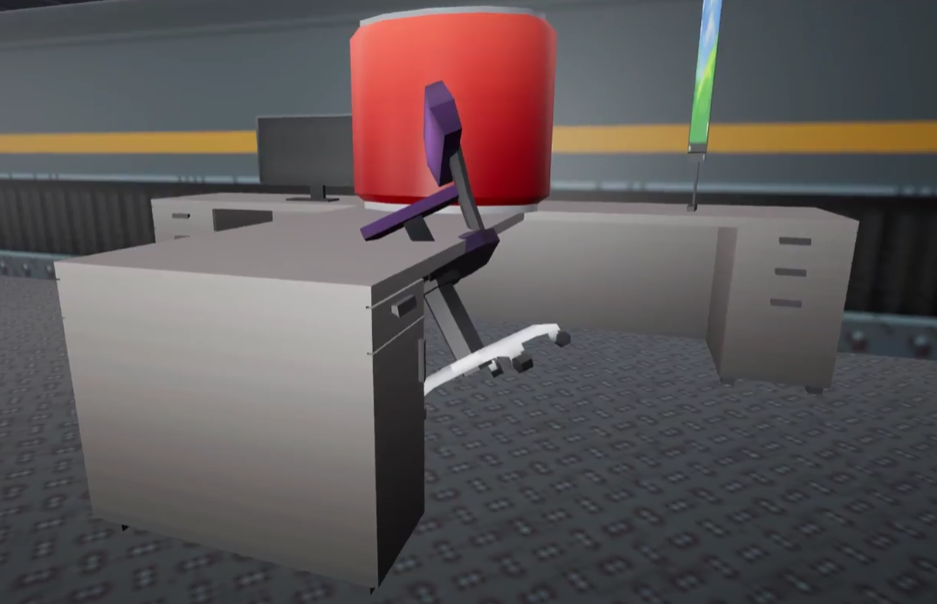
\includegraphics[width=0.4\textwidth]{timeMessedUp.png}
\captionof{figure}{In-game representation of time distortion.}
    \label{fig:time-dist}
\end{center}


\section{Art Style}
When creating our game, we wanted to try making something that felt similar to \textit{DOOM (1993)}, \textit{Paranautical Activity}, and other retro feeling games. This led to it featuring a mashup of a 2D and 3D art style. The world itself is crafting using 3D objects, but the enemies and items are represented as hand-crafted 2D sprites that always face the player. This creates an atmosphere like none other than we have experienced in a VR game. While our sprites don’t encompass what is seen in games like \textit{DOOM}, where the enemy sprites actually turn away from the player based on their movement, we feel that it created a different style that feels like an homage rather than a copy.
\begin{center}
    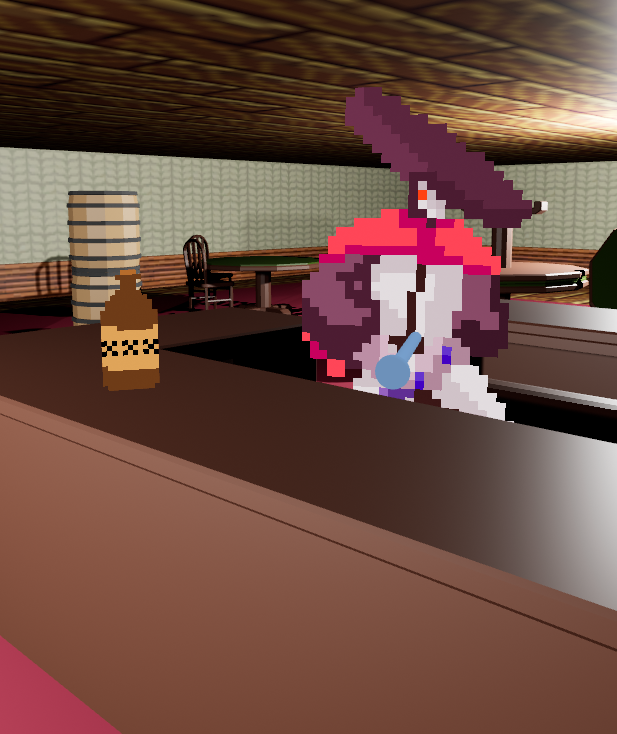
\includegraphics[width=0.3\textwidth]{2D.png}
\captionof{figure}{2D enemy and item sprites placed in the 3D world.}
    \label{fig:2D}
\end{center}

\subsubsection*{Creating Sprites}
Because we were unable to find any front-facing sprites on itch.io \cite{itch} or anywhere else, I created five of the six enemy sprites found in the game. I am not an artist so it was a challenge trying to make the sprites look presentable to some degree. My limited experience is evident when looking at the sprite and seeing choppy animation work. This is because I did not create many frames for each animation. 
\begin{center}
    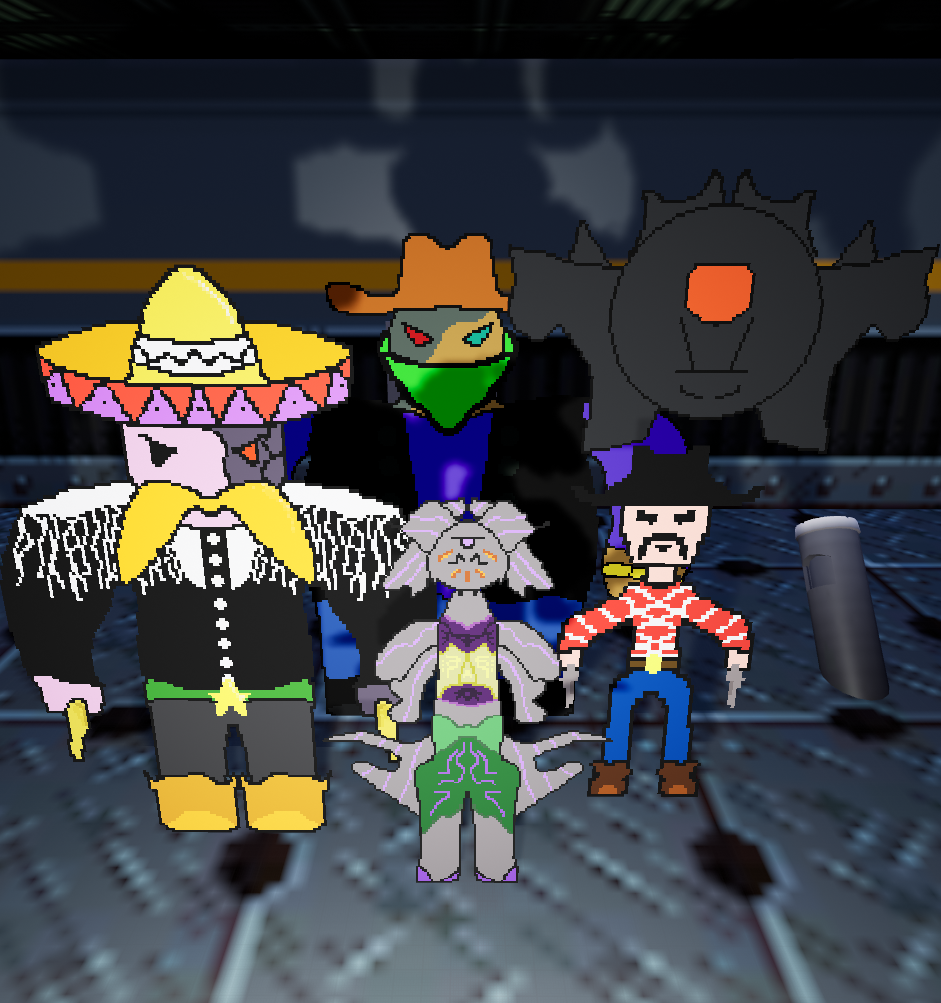
\includegraphics[width=0.35\textwidth]{sprite.png}
\captionof{figure}{All of the enemy sprites that were handmade.}
    \label{fig:Sprites}
\end{center}

\section{Technical Specifications}
The project is built with Unreal Engine 5 \cite{unrealweb} and we used Unreal's Blueprints, a visual programming language, to create the logic of the game. We use a plugin called Procedural Dungeon Plugin \cite{dungeonplugin} that places the rooms into a playable layout. To plan our roadmap we used Milanote \cite{milanote}. The assets we have in our project come from Humble Bundle \cite{humble} and itch.io \cite{itch}. As for source control, we used Git LFS \cite{gitlfs}, which is used for large files on github, and the built-in source control for Unreal Engine.

\section{Overview of Mechanics}
From the start of our project's lifespan, we wanted procedural generation in our game because we wanted to construct a VR roguelike video game. There are several different ways of handling procedural generation and we chose the procedural generation of level layouts. Kronos offers two methods of movement: head-based locomotion and hand-based locomotion. The locomotion moves like a standard video game in which you hold the movement button to move in your desired direction. Head-based locomotion uses the direction of where the player is facing in order to determine the direction of movement, while hand-based locomotion uses the direction of the left hand. The enemies' behavior (AI) was implemented using Unreal's Blueprints. Similar to most video games, each level is concluded by defeating a boss enemy that is stronger than the enemies you have been fighting on the current floor. There are multiple weapons, items that affect your player's stats, background audio, and a variety of enemies on each floor.

\section{Experiences}
\subsection*{Weapons}
When we first decided to create a VR game, research was immediately started on how to import and use a low-poly weapon. It was overwhelming at first because we had never developed with any game engine, but it became easier as we read Epic's documentation on the subject. The most difficult part of getting a weapon to work was finding a decent muzzle fire animation. The focus of our project changed immediately to prioritize building the base mechanics first like movement to ensure we have a playable game.

\subsection*{Locomotion Movement}
Unreal Engine’s built-in VRPawn object is created with a teleportation-style movement instead of the smooth movement you would expect from a standard 3D video game. Adding smooth locomotion to the game allowed us to learn a lot about the Blueprints scripting language. We were also able to learn about events, adding different elements to the viewport that aid with player location detection that are not visible to the player, and different custom collision descriptions. In the process of adding this, we ran into one major problem, collision. The default collision provided by Unreal led to the player being moved while holding an item due to the addition of smooth locomotion. Once the collision had been sorted, it was time to move to the next feature, enemies. 

\subsubsection*{Procedural Generation}
In order to make a rogue-like game, Kronos needed to have procedural generation. We both wanted the generation of levels to be similar to how The Binding of Isaac's system works. This type of generation places levels together randomly until a valid dungeon is created. A valid dungeon is when there is a start level, an end level, and a number of levels that connect the start and end level together. Instead of creating a system that places the levels for us, we decided to search if Unreal had a built-in system for this. Unreal did not have a free plugin available, but there is a free plugin on GitHub called Procedural Dungeon Plugin by BenPyton. This plugin had exactly what we were looking for. The plugin allows you to set the minimum and maximum amount of levels between the start and finish since you would want to have a cap on the amount of rooms on a level, otherwise the plugin would be adding levels forever. Because this plugin is not provided by Unreal, it was difficult to get it working with our project. Because the plugin was built using a third person character, there was some trouble setting it up with Kronos since it is set in VR. For example, it was difficult trying to find out how to teleport the player to the generated level. After getting the player in the dungeon, we ran into the generated dungeon only showing the first two rooms, which led to several hours trying to troubleshoot on why that was occurring. Eventually we decide to check the plugin's issues tab on GitHub and found a ticket that had a similar problem. The author of the plugin resolved their issue and we were able to fix the visibility of our dungeon by disabling a single setting called ''Occlusion Culling`` in the plugin's settings. The author had it enabled on default for performance purposes, but this was not needed for testing and debugging.
\begin{center}
    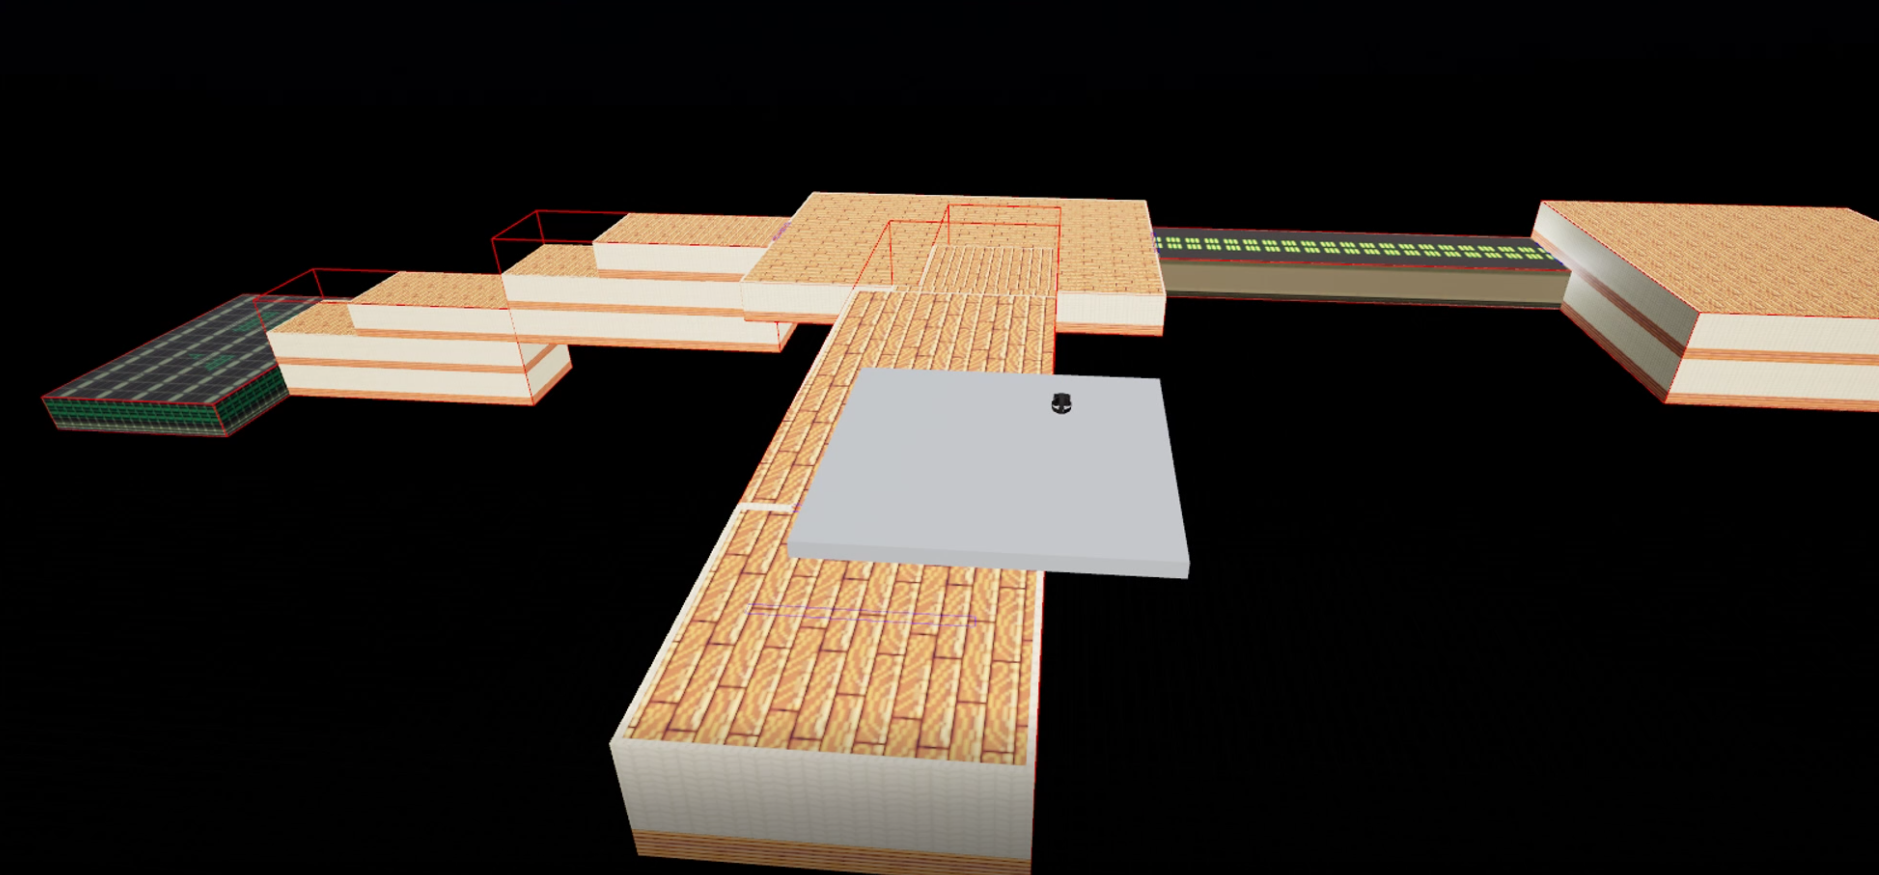
\includegraphics[width=0.45\textwidth]{dungeon.png}
\captionof{figure}{A fully generated dungeon after the procedural dungeon plugin is finished running.}
    \label{fig:Sprites}
\end{center}

\subsubsection*{Enemies} Because there were not free available sprites that fit our game's art style, we created sprites and flipbooks to make an animation for our 2D enemies. This also gave us a chance to experiment with behavior trees to allow for the AI to function on its own. Prior to the decision to use behavior trees, the behavior of the AI was created entirely through Blueprints. This caused a lot of issues, especially when it came to handling animations. Occasionally, the enemy would change their sprite while another event would occur, stopping the enemy’s sprite from reflecting their current action. 

\subsubsection*{Artificial Intelligence} Implementing the AI was where the majority of our time was spent since there were many issues. There was so much to learn about AI and this resulted in us learning the ins and outs of Behavior Trees in Unreal Engine. In the beginning, the AI could move randomly in a specified radius. This little introduction allowed us to learn about the little pieces that are needed to make an AI in Unreal. Then moved onto Unreal's Blackboard, which is an object that holds all the values, in variables, that a single instance of an AI needs to function. The next step was AI Controllers, which is where you determine the Behavior Tree that needs to be run. This attaches senses to the enemies, so they could visually analyze their surroundings to look for the player. AI Controllers can also talk to the Blackboard to change values based on these senses that may be helpful for AI behaviors. Finally, we have the Behavior Trees. These look just like what you would see with regular trees in computer science. When working with the actual Behavior Trees, there are three main elements that were used: selectors, sequences, and tasks. Selectors run the first child node that does not fail to run properly. Sequences run each child node from left to right until one of them fails or all children have been executed, which stops the sequence and returns to its parent node. Tasks are the actual functionality of the AI. This includes things like attacking, finding the player location, moving, and more. All these pieces combine to make an AI that can make informed decisions based on its senses.

\subsubsection*{Items} In order to create items, we considered everything that would be needed so that all the pieces make a working item. This included the objects that the player can collect, the spawning mechanism for the items, and the 2D sprites for the items. This allowed for us to learn about how to spawn objects in the game through the Blueprints system. Not only that, but we were also able to learn about the randomness that Unreal can provide for random selection.

\subsubsection*{Weapons... Again}
After creating the core mechanics of the game, the focus of the project shifted back to weapons. There were plenty of issues trying to allow the player to grab a weapon with both hands so we decided to only have one-handed weapons. Getting a two-handed weapon to work in VR would require a skeleton for the weapon and we were unable to create a skeleton with the weapon models already in the project. This was likely because our imported models did not have a skeleton. A skeleton would allow for bones to be created, meaning there are two bones for where each hand could be placed on the weapon. The decision to only have one-handed weapons was made for the sake of time and trying to get the game to a playable state first.

\subsubsection*{Audio}
Importing and adding music to our Unreal project was surprisingly easy. We decided that we wanted a retro tone to our game so we used a 16-bit music pack from Humble Bundle \cite{humble}. This was used for the background music to our levels. We also added footstep and gunshot sounds that also were from Humble \cite{humble}. We were unable to find an audio clip that could be used for our player taking damage so we did not incorporate it into our game. 

\section{Trials and Tribulations}
Throughout the creation of Kronos, we ran into some troubles that slowed down progression. 
\subsection*{Locomotion Movement}
Initially, getting the locomotion movement to work without issue was troublesome. This issue arose with making objects able to be grabbed. Grabbing lead to a dive through collision to understand how Unreal processed what should collide with what and what to do upon colliding. The most common issue we experienced with grabbing was the case where the player would grab an object, which would then collide with the player's collision detection, moving the player in the opposite direction of the held object. Luckily, this was able to be fixed after learning more about collision presets.
\subsection*{Sprite Changing}
Another problem we faced was sprite handling. As the enemies moved, attacked, took damage, and more, we wanted the sprite to update to represent this. Originally, we were creating our enemies through the Blueprint system alone. This meant that we were handling all sorts of events, and keeping up with what the enemy should be displaying. This wasn't a problem until multiple events fired at the same time. The firing of multiple events led to sprites not being updated or getting updated to the wrong sprite for the action. This was undesirable, so some research needed to be done. Since this was a niche style of enemy, there was not much help available for us in this regard. During our research though, we learned about behavior trees for AI and how to implement them. This allowed for us to put more of the work and thinking on the built-in AI system in Unreal instead of creating our own and essentially recreating the wheel. Using Behavior Trees also just happened to solve our sprite problems, so it ended up being majorly beneficial.
\subsection*{Procedural Dungeon Plugin}
There were several issues with using the procedural dungeon plugin, which is a third-party plugin. To begin with, the plugin was built using a first-person player and did not allow for a VRplayer pawn to be used as easy. This was troubling at first because our entire idea of Kronos was to create a VR roguelike and not a first-person shooter.After sorting that issue, our progress came to a halt once we realized that the player and enemy were unable to move in the generated dungeon.  This was due to the navigation mesh, which is what defines where a player and enemy can move to. The problem was that the navigation mesh did not rebuild itself when the dungeon was being generated. The resolution to this error was to enable a setting in the project's settings and allowed a dynamic navigation mesh.

\section{Conclusions}
At the end of the project, we are able to walk away with a lot of new knowledge. Over the course of development, we learned how to use Unreal Engine 5 and many of the features it offers. We learned more about visual scripting languages through Blueprints. We were able to experience world creation, AI behaviors, making sprites through pixel art, and much more. Overall, this has been a useful learning experience. Even if we don't make much use of these skills going forward in our careers, it will always be something can feel free to dabble with on our own time.

\section{Future Work}
As we move forward with the creation of Kronos, we have a couple of ideas in mind to flesh out. We would like to add a new floor, likely a modern era. With this, we would like to add more enemies and bosses to add variety to the enemies. Along with new enemies, we would want to refine our AI in order to create more intelligent behaviors to add depth to the gameplay. For example, implementing a cover system in which the AI looks for cover to hide behind while below 50\% health. We would also like to create more items and possibly ways to earn items to further support the ability to continue to play new playthroughs without the experience getting stale. Finally, incorporating a save system is something we wanted to implement from the beginning but couldn't because of difficulties introduced by the procedural dungeon plugin we chose to use. Adding a save system would be difficult to implement because the dungeon is generated at runtime and does not save the player's stats, enemies, player and enemies' locations, and more. At first we tried getting a save system to work, but due to deadlines, we focused our attention on getting to a playable state first.

%\section{Page Size and Columns}
%On each page your material should fit within a rectangle of 7 $\times$
%9.15 inches (18 $\times$ 23.2 cm), centered on a US Letter page (8.5
%$\times$ 11 inches), beginning 0.85 inches (1.9 cm) from the top of
%the page, with a 0.3 inches (0.85 cm) space between two 3.35 inches
%(8.4 cm) columns. Right margins should be justified, not
%ragged. Please be sure your document and PDF are US letter and not A4.
%
%\section{Typeset Text}
%The styles contained in this document have been modified from the
%default styles to reflect ACM formatting conventions. For example,
%content paragraphs like this one are formatted using the Normal style.
%
%\LaTeX\ sometimes will create overfull lines that extend into columns.
%To attempt to combat this, the \texttt{.cls} file has a command,
%\texttt{{\textbackslash}sloppy}, that essentially asks \LaTeX\ to
%prefer underfull lines with extra whitespace.  For more details on
%this, and info on how to control it more finely, check out
%{\url{http://www.economics.utoronto.ca/osborne/latex/PMAKEUP.HTM}}.
%
%\subsection{Title and Authors}
%
%Your paper's title, authors and affiliations should run across the
%full width of the page in a single column 17.8 cm (7 in.) wide.  The
%title should be in Helvetica or Arial 18-point bold.  Authors' names
%should be in Times New Roman or Times Roman 12-point bold, and
%affiliations in 12-point regular.  
%
%See \texttt{{\textbackslash}author} section of this template for
%instructions on how to format the authors. For more than three
%authors, you may have to place some address information in a footnote,
%or in a named section at the end of your paper. Names may optionally
%be placed in a single centered row instead of at the top of each
%column. Leave one 10-point line of white space below the last line of
%affiliations.
%
%\subsection{Abstract and Keywords}
%
%Every submission should begin with an abstract of about 150 words,
%followed by a set of Author Keywords and ACM Classification
%Keywords. The abstract and keywords should be placed in the left
%column of the first page under the left half of the title. The
%abstract should be a concise statement of the problem, approach, and
%conclusions of the work described. It should clearly state the paper's
%contribution to the field of HCI\@.
%
%\subsection{Normal or Body Text}
%
%Please use a 10-point Times New Roman or Times Roman font or, if this
%is unavailable, another proportional font with serifs, as close as
%possible in appearance to Times Roman 10-point. Other than Helvetica
%or Arial headings, please use sans-serif or non-proportional fonts
%only for special purposes, such as source code text.
%
%\subsection{First Page Copyright Notice}
%This template include a sample ACM copyright notice at the bottom of
%page 1, column 1.  Upon acceptance, you will be provided with the
%appropriate copyright statement and unique DOI string for publication.
%Accepted papers will be distributed in the conference
%publications. They will also be placed in the ACM Digital Library,
%where they will remain accessible to thousands of researchers and
%practitioners worldwide. See
%\url{http://acm.org/publications/policies/copyright_policy} for the
%ACM's copyright and permissions policy.
%
%\subsection{Subsequent Pages}
%
%On pages beyond the first, start at the top of the page and continue
%in double-column format.  The two columns on the last page should be
%of equal length.
%
%%% \begin{figure}
%%% \centering
%%%   \includegraphics[width=0.9\columnwidth]{figures/sigchi-logo}
%%%   \caption{Insert a caption below each figure. Do not alter the
%%%     Caption style.  One-line captions should be centered; multi-line
%%%     should be justified. }~\label{fig:figure1}
%%% \end{figure}
%
%\subsection{References and Citations}
%
%Use a numbered list of references at the end of the article, ordered
%alphabetically by last name of first author, and referenced by numbers
%in
%brackets~\cite{acm_categories,ethics,Klemmer:2002:WSC:503376.503378}.
%Your references should be published materials accessible to the
%public. Internal technical reports may be cited only if they are
%easily accessible (i.e., you provide the address for obtaining the
%report within your citation) and may be obtained by any reader for a
%nominal fee. Proprietary information may not be cited. Private
%communications should be acknowledged in the main text, not referenced
%(e.g., ``[Borriello, personal communication]'').
%
%References should be in ACM citation format:
%\url{http://acm.org/publications/submissions/latex_style}. This
%includes citations to internet
%resources~\cite{acm_categories,cavender:writing,CHINOSAUR:venue,psy:gangnam}
%according to ACM format, although it is often appropriate to include
%URLs directly in the text, as above.
%
%
%% Use a numbered list of references at the end of the article, ordered
%% alphabetically by first author, and referenced by numbers in
%% brackets~\cite{ethics, Klemmer:2002:WSC:503376.503378,
%%   Mather:2000:MUT, Zellweger:2001:FAO:504216.504224}. For papers from
%% conference proceedings, include the title of the paper and an
%% abbreviated name of the conference (e.g., for Interact 2003
%% proceedings, use \textit{Proc. Interact 2003}). Do not include the
%% location of the conference or the exact date; do include the page
%% numbers if available. See the examples of citations at the end of this
%% document. Within this template file, use the \texttt{References} style
%% for the text of your citation.
%
%% Your references should be published materials accessible to the
%% public.  Internal technical reports may be cited only if they are
%% easily accessible (i.e., you provide the address for obtaining the
%% report within your citation) and may be obtained by any reader for a
%% nominal fee.  Proprietary information may not be cited. Private
%% communications should be acknowledged in the main text, not referenced
%% (e.g., ``[Robertson, personal communication]'').
%
%\begin{table}
%  \centering
%  \begin{tabular}{l r r r}
%    % \toprule
%    & & \multicolumn{2}{c}{\small{\textbf{Test Conditions}}} \\
%    \cmidrule(r){3-4}
%    {\small\textit{Name}}
%    & {\small \textit{First}}
%      & {\small \textit{Second}}
%    & {\small \textit{Final}} \\
%    \midrule
%    Marsden & 223.0 & 44 & 432,321 \\
%    Nass & 22.2 & 16 & 234,333 \\
%    Borriello & 22.9 & 11 & 93,123 \\
%    Karat & 34.9 & 2200 & 103,322 \\
%    % \bottomrule
%  \end{tabular}
%  \caption{Table captions should be placed below the table. We
%    recommend table lines be 1 point, 25\% black. Minimize use of
%    table grid lines.}~\label{tab:table1}
%\end{table}
%
%\section{Sections}
%
%The heading of a section should be in Helvetica or Arial 9-point bold,
%all in capitals. Sections should \textit{not} be numbered.
%
%\subsection{Subsections}
%
%Headings of subsections should be in Helvetica or Arial 9-point bold
%with initial letters capitalized.  For sub-sections and
%sub-subsections, a word like \emph{the} or \emph{of} is not
%capitalized unless it is the first word of the heading.
%
%\subsubsection{Sub-subsections}
%
%Headings for sub-subsections should be in Helvetica or Arial 9-point
%italic with initial letters capitalized.  Standard
%\texttt{{\textbackslash}section}, \texttt{{\textbackslash}subsection},
%and \texttt{{\textbackslash}subsubsection} commands will work fine in
%this template.
%
%\section{Figures/Captions}
%
%Place figures and tables at the top or bottom of the appropriate
%column or columns, on the same page as the relevant text (see
%Figure~\ref{fig:figure1}). A figure or table may extend across both
%columns to a maximum width of 17.78 cm (7 in.).
%
%%% \begin{figure*}
%%%   \centering
%%%   \includegraphics[width=1.75\columnwidth]{figures/map}
%%%   \caption{In this image, the map maximizes use of space. You can make
%%%     figures as wide as you need, up to a maximum of the full width of
%%%     both columns. Note that \LaTeX\ tends to render large figures on a
%%%     dedicated page. Image: \ccbynd~ayman on
%%%     Flickr.}~\label{fig:figure2}
%%% \end{figure*}
%
%Captions should be Times New Roman or Times Roman 9-point bold.  They
%should be numbered (e.g., ``Table~\ref{tab:table1}'' or
%``Figure~\ref{fig:figure1}''), centered (if one line) otherwise justified, and placed beneath the figure
%or table.  Please note that the words ``Figure'' and ``Table'' should
%be spelled out (e.g., ``Figure'' rather than ``Fig.'') wherever they
%occur. Figures, like Figure~\ref{fig:figure2}, may span columns and
%all figures should also include alt text for improved accessibility.
%Papers and notes may use color figures, which are included in the page
%limit; the figures must be usable when printed in black-and-white in
%the proceedings.
%
%The paper may be accompanied by a short video figure (we recommend staying within five
%minutes in length). However, the paper should stand on its own without
%the video figure, as the video may not be available to everyone who
%reads the paper.  
%
%\subsection{Inserting Images}
%When possible, include a vector formatted graphic (i.e. PDF or EPS).
%When including bitmaps,  use an image editing tool to resize the image
%at the appropriate printing resolution (usually 300 dpi).
%
%\section{Quotations}
%Quotations may be italicized when \textit{``placed inline''}.
%
%\begin{quote}
%Longer quotes, when placed in their own paragraph, need not be
%italicized or in quotation marks when indented.  
%\end{quote}
%
%\section{Language, Style, and Content}
%
%The written and spoken language of SIGCHI is English. Spelling and
%punctuation may use any dialect of English (e.g., British, Canadian,
%US, etc.) provided this is done consis- tently. Hyphenation is
%optional. To ensure suitability for an international audience, please
%pay attention to the following:
%
%\begin{itemize}
%\item Write in a straightforward style.
%\item Try to avoid long or complex sentence structures.
%\item Use common and basic vocabulary (e.g., use the word ``unusual'' rather than the word ``arcane''.
%\item Briefly define or explain all technical terms that may be
%  unfamiliar to readers.
%\item Explain all acronyms the first time they are used in your
%  text---e.g., ``Digital Signal Processing (DSP)''.
%\item Explain local references (e.g., not everyone knows all city
%  names in a particular country).
%\item Explain ``insider'' comments. Ensure that your whole audience
%  understands any reference whose meaning you do not describe (e.g.,
%  do not assume that everyone has used a Macintosh or a particular
%  application).
%\item Explain colloquial language and puns. Understanding phrases like
%  ``red herring'' may require a local knowledge of English.  Humor and
%  irony are difficult to translate.
%\item Use unambiguous forms for culturally localized concepts, such as
%  times, dates, currencies, and numbers (e.g., ``1--5--97'' or
%  ``5/1/97'' may mean 5 January or 1 May, and ``seven o'clock'' may
%  mean 7:00 am or 19:00). For currencies, indicate equivalences:
%  ``Participants were paid {\fontfamily{txr}\selectfont \textwon}
%  25,000, or roughly US \$22.''
%\item Be careful with the use of gender-specific pronouns (he, she)
%  and other gendered words (chairman, manpower, man-months). Use
%  inclusive language that is gender-neutral (e.g., she or he, they,
%  s/he, chair, staff, staff-hours, person-years). See the
%  \textit{Guidelines for Bias-Free Writing} for further advice and
%  examples regarding gender and other personal
%  attributes~\cite{Schwartz:1995:GBF}. Be particularly aware of
%  considerations around writing about people with disabilities.
%\item If possible, use the full (extended) alphabetic character set
%  for names of persons, institutions, and places (e.g.,
%  Gr{\o}nb{\ae}k, Lafreni\'ere, S\'anchez, Nguy{\~{\^{e}}}n,
%  Universit{\"a}t, Wei{\ss}enbach, Z{\"u}llighoven, \r{A}rhus, etc.).
%  These characters are already included in most versions and variants
%  of Times, Helvetica, and Arial fonts.
%\end{itemize}
%
%\section{Accessibility}
%The Executive Council of SIGCHI has committed to making SIGCHI
%conferences more inclusive for researchers, practitioners, and
%educators with disabilities. As a part of this goal, the all authors
%are asked to work on improving the accessibility of their
%submissions. Specifically, we encourage authors to carry out the
%following five steps:
%\begin{enumerate}
%\item Add alternative text to all figures
%\item Mark table headings
%\item Add tags to the PDF
%\item Verify the default language
%\item Set the tab order to ``Use Document Structure''
%\end{enumerate}
%For more information and links to instructions and resources, please
%see: \url{http://chi2016.acm.org/accessibility}.  The
%\texttt{{\textbackslash}hyperref} package allows you to create well tagged PDF files,
%please see the preamble of this template for an example.
%
%\section{Page Numbering, Headers and Footers}
%Your final submission should not contain footer or header information
%at the top or bottom of each page. Specifically, your final submission
%should not include page numbers. Initial submissions may include page
%numbers, but these must be removed for camera-ready. Page numbers will
%be added to the PDF when the proceedings are assembled.
%
%\section{Producing and Testing PDF Files}
%
%We recommend that you produce a PDF version of your submission well
%before the final deadline.  Your PDF file must be ACM DL
%Compliant. The requirements for an ACM Compliant PDF are available at:
%{\url{http://www.scomminc.com/pp/acmsig/ACM-DL-pdfs-requirements.htm}}.
%
%Test your PDF file by viewing or printing it with the same software we
%will use when we receive it, Adobe Acrobat Reader Version 10. This is
%widely available at no cost. Note that most
%reviewers will use a North American/European version of Acrobat
%reader, so please check your PDF accordingly.
%
%\section{Conclusion}
%
%It is important that you write for the SIGCHI audience. Please read
%previous years' proceedings to understand the writing style and
%conventions that successful authors have used. It is particularly
%important that you state clearly what you have done, not merely what
%you plan to do, and explain how your work is different from previously
%published work, i.e., the unique contribution that your work makes to
%the field. Please consider what the reader will learn from your
%submission, and how they will find your work useful. If you write with
%these questions in mind, your work is more likely to be successful,
%both in being accepted into the conference, and in influencing the
%work of our field.
%
%\section{Acknowledgments}
%
%Sample text: We thank all the volunteers, and all publications support
%and staff, who wrote and provided helpful comments on previous
%versions of this document. Authors 1, 2, and 3 gratefully acknowledge
%the grant from NSF (\#1234--2012--ABC). \textit{This whole paragraph is
%  just an example.}
%
%% Balancing columns in a ref list is a bit of a pain because you
%% either use a hack like flushend or balance, or manually insert
%% a column break.  http://www.tex.ac.uk/cgi-bin/texfaq2html?label=balance
%% multicols doesn't work because we're already in two-column mode,
%% and flushend isn't awesome, so I choose balance.  See this
%% for more info: http://cs.brown.edu/system/software/latex/doc/balance.pdf
%%
%% Note that in a perfect world balance wants to be in the first
%% column of the last page.
%%
%% If balance doesn't work for you, you can remove that and
%% hard-code a column break into the bbl file right before you
%% submit:
%%
%% http://stackoverflow.com/questions/2149854/how-to-manually-equalize-columns-
%% in-an-ieee-paper-if-using-bibtex
%%
%% Or, just remove \balance and give up on balancing the last page.
%%
%\balance{}
%
%\section{References Format}
%Your references should be published materials accessible to the
%public. Internal technical reports may be cited only if they are
%easily accessible and may be obtained by any reader for a nominal
%fee. Proprietary information may not be cited. Private communications
%should be acknowledged in the main text, not referenced (e.g.,
%[Golovchinsky, personal communication]). References must be the same
%font size as other body text. References should be in alphabetical
%order by last name of first author. Use a numbered list of references
%at the end of the article, ordered alphabetically by last name of
%first author, and referenced by numbers in brackets. For papers from
%conference proceedings, include the title of the paper and the name of
%the conference. Do not include the location of the conference or the
%exact date; do include the page numbers if available. 
%
%References should be in ACM citation format:
%\url{http://www.acm.org/publications/submissions/latex_style}.  This
%includes citations to Internet
%resources~\cite{CHINOSAUR:venue,cavender:writing,psy:gangnam}
%according to ACM format, although it is often appropriate to include
%URLs directly in the text, as above. Example reference formatting for
%individual journal articles~\cite{ethics}, articles in conference
%proceedings~\cite{Klemmer:2002:WSC:503376.503378},
%books~\cite{Schwartz:1995:GBF}, theses~\cite{sutherland:sketchpad},
%book chapters~\cite{winner:politics}, an entire journal
%issue~\cite{kaye:puc},
%websites~\cite{acm_categories,cavender:writing},
%tweets~\cite{CHINOSAUR:venue}, patents~\cite{heilig:sensorama}, 
%games~\cite{supermetroid:snes}, and
%online videos~\cite{psy:gangnam} is given here.  See the examples of
%citations at the end of this document and in the accompanying
%\texttt{BibTeX} document. This formatting is a edited version of the
%format automatically generated by the ACM Digital Library
%(\url{http://dl.acm.org}) as ``ACM Ref.'' DOI and/or URL links are
%optional but encouraged as are full first names. Note that the
%Hyperlink style used throughout this document uses blue links;
%however, URLs in the references section may optionally appear in
%black.
%
%% BALANCE COLUMNS
%\balance{}
%
%% REFERENCES FORMAT
%% References must be the same font size as other body text.
%\bibliographystyle{SIGCHI-Reference-Format}
%\bibliography{sample}

\bibliographystyle{plain}
\bibliography{bibliography}
\end{document}


